\documentclass{article}
\setlength{\parindent}{0pt}
\usepackage{fullpage}
\usepackage{graphicx} % Required for inserting images
\usepackage{biblatex}
\usepackage{listings}
\usepackage[section]{placeins}
\usepackage{float}
\lstset{
  basicstyle=\footnotesize\ttfamily,
  breaklines=true,
  escapeinside={\%*}{*)},
  extendedchars=true,
  keepspaces=true,
  showstringspaces=false,
}


\title{Unicity: Autonomous Agent-Based Decentralized Applications}
\author{The Unicity Developers\\unicity-devs@proton.me}
\date{}

\begin{document}
\maketitle



\begin{abstract}
\noindent  Unicity is a new blockchain platform for the development of scalable decentralized applications based on a network of verifiable autonomous agents. The key innovation is to disaggregate the uniqueness (non-forking) proof for the blockchain as a whole, allowing uniqueness proofs to be generated for individual agents executing in parallel off-chain. This removes two of the key scaling bottlenecks; there is no restriction on size as agents are not stored on-chain and there is no restriction on compute as  agents execute locally in their own environments. Agents interact by synchronizing provably unique state histories. As all computation happens in parallel off-chain, practically unlimited throughput can be achieved. Unicity acts as a decentralized microservices platform, breaking down a decentralized application into small independent agents that can be developed, deployed and scaled without a centralized gatekeeper.
\end{abstract}

\section*{TL;DR}



\begin{itemize}

  \setlength{\leftmargin}{1em}
  
 \item Agent: an encapsulation of code and state that receives inputs from an external environment, executes its code and updates its state and code accordingly.
 \item Public permissionless blockchain architecture for off-chain parallel execution of verifiable agents. Agents interact autonomously to execute scalable decentralized applications.
 \item  Three layers: Proof of Work (PoW) consensus, Proof Aggregation and Agent Layers.
\item PoW Layer: Native platform currency(ALPHA) and global trust anchor. RandomX ASIC resistant hash function ensuring fair mining and decentralization. Two minute block times, 10 ALPHA subsidy per block. Exponential moving average difficulty adjustment. Zero pre-mine.
\item  Block reward winners form a subset of miners that operate a finality gadget and BFT consensus subnet with one second block times. 
\item Only single input UTXOs are allowed by consensus rules enabling decomposition of the ledger into compact individual coin sub-ledgers, which can then be extracted and used by agents in the Agent Layer.
\item Proof Aggregation Layer: public permissionless infrastructure, operating an append-only fault tolerant Sparse Merkle Tree (SMT). The SMT receives requests in rounds with each round root hash value anchored in PoW layer. ZK succinct proofs of non-deletion at periodic checkpoints.
\item The SMT tree is built hierarchically. State transition requests from agents are recorded in the tree with proofs of inclusion and non-deletion providing a proof of uniqueness for agent state histories.
\item Agent Layer: Acts as a decentralized microservices platfrom providing the tools to developers to interface with the Unicity Infrastructure and develop, deploy and scale agents. As all execution is local any programming language or development environment can be used.
\end{itemize}


\section{Introduction}


\textbf{why decentralization?}
\vspace{2mm}

Blockchains and decentralization are tools, not end goals in themselves. They are means to achieve specific objectives that may not be feasible or optimal in centralized systems. Bitcoin, for example, uses decentralization as a means to achieve censorship resistance and the elimination of trusted third parties in transfer of value across the Internet. By removing central points of control decentralized applications (DApps) can create solutions that offer enhanced trust, transparency, and user empowerment. DApps can provide services that are resistant to censorship, manipulation, and single points of failure. They can enable new business models and forms of collaboration that were previously impossible or impractical. However, it's crucial to recognize that decentralization comes with trade-offs, such as potential decreases in efficiency or increased complexity.
\vspace{2mm}

In particular, the current approach used to build DApps through blockchain based smart contracts comes with enormous overhead. Current blockchains all need sequential block production and require consensus over global state.  This creates a bottleneck that limits performance and struggles to meet the performance demands of truly global, high-throughput systems. To put it bluntly, no-one is running Call of Duty or Fully Self-Driving software in a smart contract today.

\vspace{2mm}
\textbf{blockchain as a computer}
\vspace{2mm}

A blockchain can be thought of as a proof generation machine. Conceptually, it is a distributed computational machine that generates cryptographic proofs of integrity, order, uniqueness, computation, ownership, and more. The machine can be centralized or decentralized, and access can be either permissioned or permissionless. Various incentive schemes can be devised to encourage users to operate parts of the machine, and the machine can be programmable to varying degrees. The evolution of this programmability has been a defining feature in blockchain design.
\vspace{2mm}

Bitcoin, while primarily designed as a peer-to-peer electronic cash system, introduced a basic form of programmability through its scripting language. This limited scripting capability allowed simple conditions, such as multi-signature requirements or time-locked transfers, to be attached to transactions. However, Bitcoin's scripting language was intentionally restricted to maintain the network's security and focus on its primary use case as a digital currency.

\vspace{2mm}

The concept of a more expansive, programmable blockchain was significantly advanced by Vitalik Buterin with the introduction of Ethereum in 2015. Buterin envisioned a "world computer" - a global, decentralized platform capable of executing arbitrary code in the form of smart contracts. This vision expanded the blockchain's role from a mere ledger of transactions to a general-purpose computational infrastructure. The progression from Bitcoin's basic scripting to Ethereum's world computer, transformed blockchains from specialized tools for cryptocurrency into general-purpose platforms for decentralized computation and application deployment.

\begin{figure}[H]
    \centering
    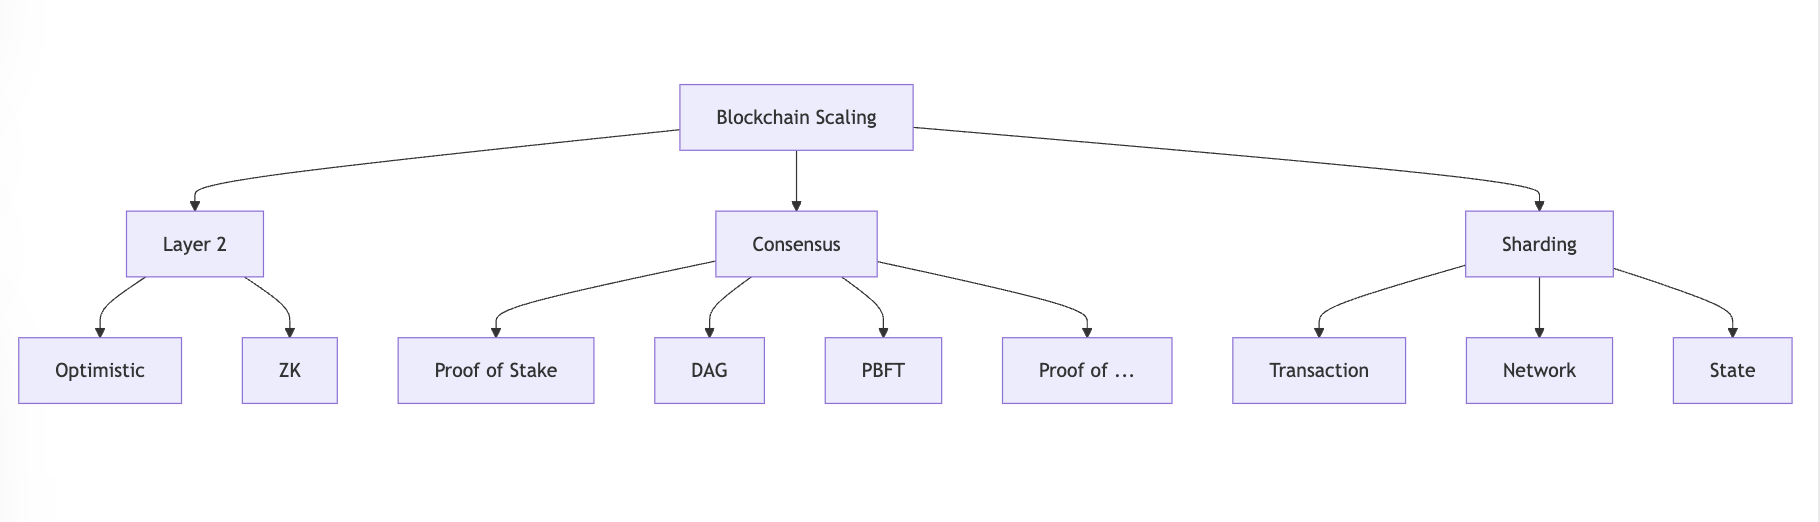
\includegraphics[width=0.9\textwidth]{scaling.png}
    \caption{Approaches to blockchain scaling }
    \label{fig:scaling}
\end{figure}


The complexity and usage of these smart contract platforms have grown, exposing fundamental limitations in their design. Blockchain computers are extremely inefficient with throughput many orders of magnitude lower than a traditional computer. Many more recent techniques have been devised to address those limitations. There are now alternative consensus protocols, layer-two solutions and sharding, which have each introduced different incremental innovations, but so far, all have turned out to be merely short-term workarounds that attempt to address the limitations of the base layer, and many are simply tradeoffs, that compromise either security or decentralization. For instance, layer-two solutions like rollups for Ethereum can increase transaction throughput by one or two orders of magnitude before they reach a hard limit. They also introduce additional complexity, centralization (centralized sequencers with escape hatches etc.) with potential security vulnerabilities at the points where they interface with the main chain. Sharding is another area of scalablity research, however it introduces new challenges in cross-shard communication that can potentially fragment the network's security model. The core issue remains: traditional blockchain architectures struggle to scale without sacrificing either security, decentralization, or both. 
\vspace{2mm}

\textbf{Unicity: disaggregating proofs of uniqueness}
\vspace{2mm}


Rather than attempting to optimize within the constraints of traditional blockchain design, Unicity introduces a fundamentally new approach to building decentralized applications. The key idea is to use verifiable autonomous agents that execute in their own environments but use the Unicity blockchain infrastructure to generate on demand uniqueness proofs of their own state histories. Proof of uniqueness or non-forking is one of the key proofs that a blockchain provides. In Bitcoin for example, Proof of Work is used to guarantee that there is a single unique version of the blockchain. The proof of uniqueness in this case is probabilistic, i.e. there may be other copies (forks) but over time the incentive scheme ensures that Miners will converge onto the chain with most work (the longest chain rule). This uniqueness proof covers all transactions in a block as all transactions are included in the Proof of Work calculation. 


\begin{figure}[htbp]
    \centering
    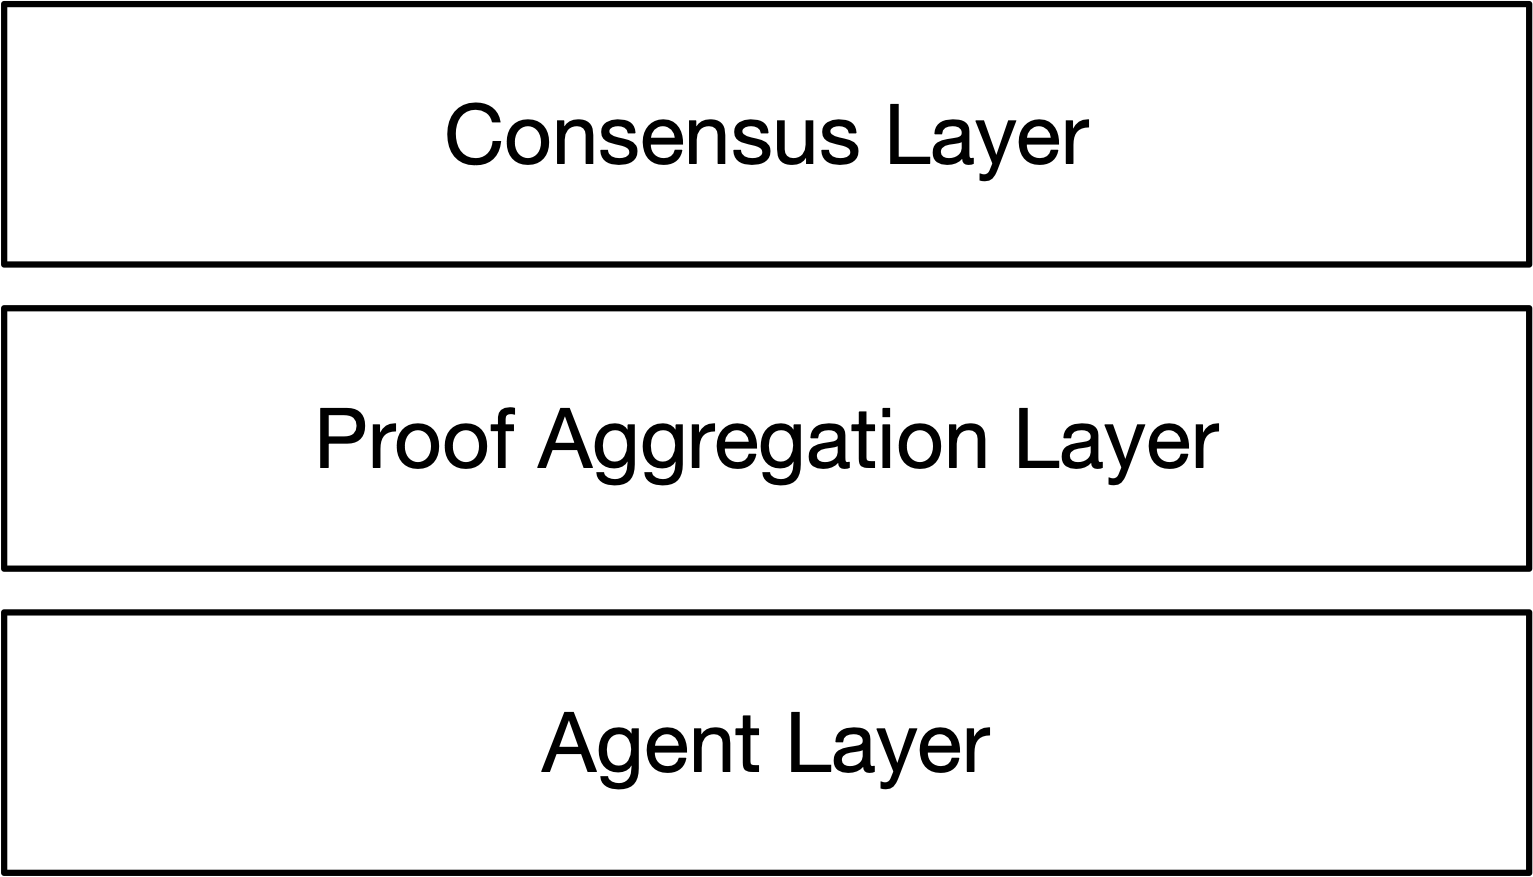
\includegraphics[width=0.4\textwidth]{ThreeLayers.png}
    \caption{Unicity Layered Infrastructure}
    \label{fig:layers}
\end{figure}


In Unicity, the Consensus Layer uses Proof of Work to provide a trust anchor to attest to uniqueness of the global state as well as for coin genesis. Although the public permissionless version of Unicity uses Proof of Work, any Proof system could be used including Proof of Stake, Proof of Authority or trusted hardware. The key difference is that transactions, or more generally \textit{state transitions}, are not included in blocks\footnote{Certain transactions are still necessary at this layer. For example coinbase transactions or the distribution of shares in mining pools.}. Instead, state transitions happen at the Agent Layer where each agent will periodically send a request to the Proof Aggregation Layer and receive back a uniqueness proof for the set of sequential state transitions that occurred during the previous period. This decoupling allows agents to independently generate proofs of uniqueness locally as if they were generated through the traditional consensus process. Crucially, it also allows Agents to perform computationally difficult work independently from the miners, which eliminates the computational bottleneck that Ethereum's global state suffers from.

\vspace{2mm}

In the following sections, we will delve into the design principles and implementation details of Unicity and then explore two key use cases that highlight the platform's capability:

\begin{itemize}
\setlength{\leftmargin}{1em}
 \item Censorship-resistant digital currency and decentralized finance:  We start with the native currency of Unicity and show how this can be used for agent to agent payments. We then develop agents that act as the building blocks for high performance decentralized exchanges and the other functions of a decentralized financial ecosystem.
 \item Decentralized gaming: Actually running a decentralized version of Call of Duty.  This was the original motivation behind this work - to implement a new form of decentralized gaming known as massive online multi-player immersive simulations.
\end{itemize}


To bring decentralized applications mainstream it is not only necessary to overcome the performance limitations but also provide a vastly improved developer experience with simple integration tools for existing applications and services. In Unicity all computation happens on the client side, simplifying the developer experience and reducing the need for new programming languages or blockchain knowledge. Any programming language can be used and existing applications can be packaged as agents  using API calls to request a proof of unique state history.


\section{Implementation: Consensus Layer}

The Alphacash public blockchain is used, both as the trust anchor and as the native currency of the system (for compensating network participants and paying of transaction fees). Alphacash is purpose built for Unicity as a zero-premine Proof of Work chain similar to Bitcoin, but with several modifications.

\begin{figure}[htbp]
    \centering
    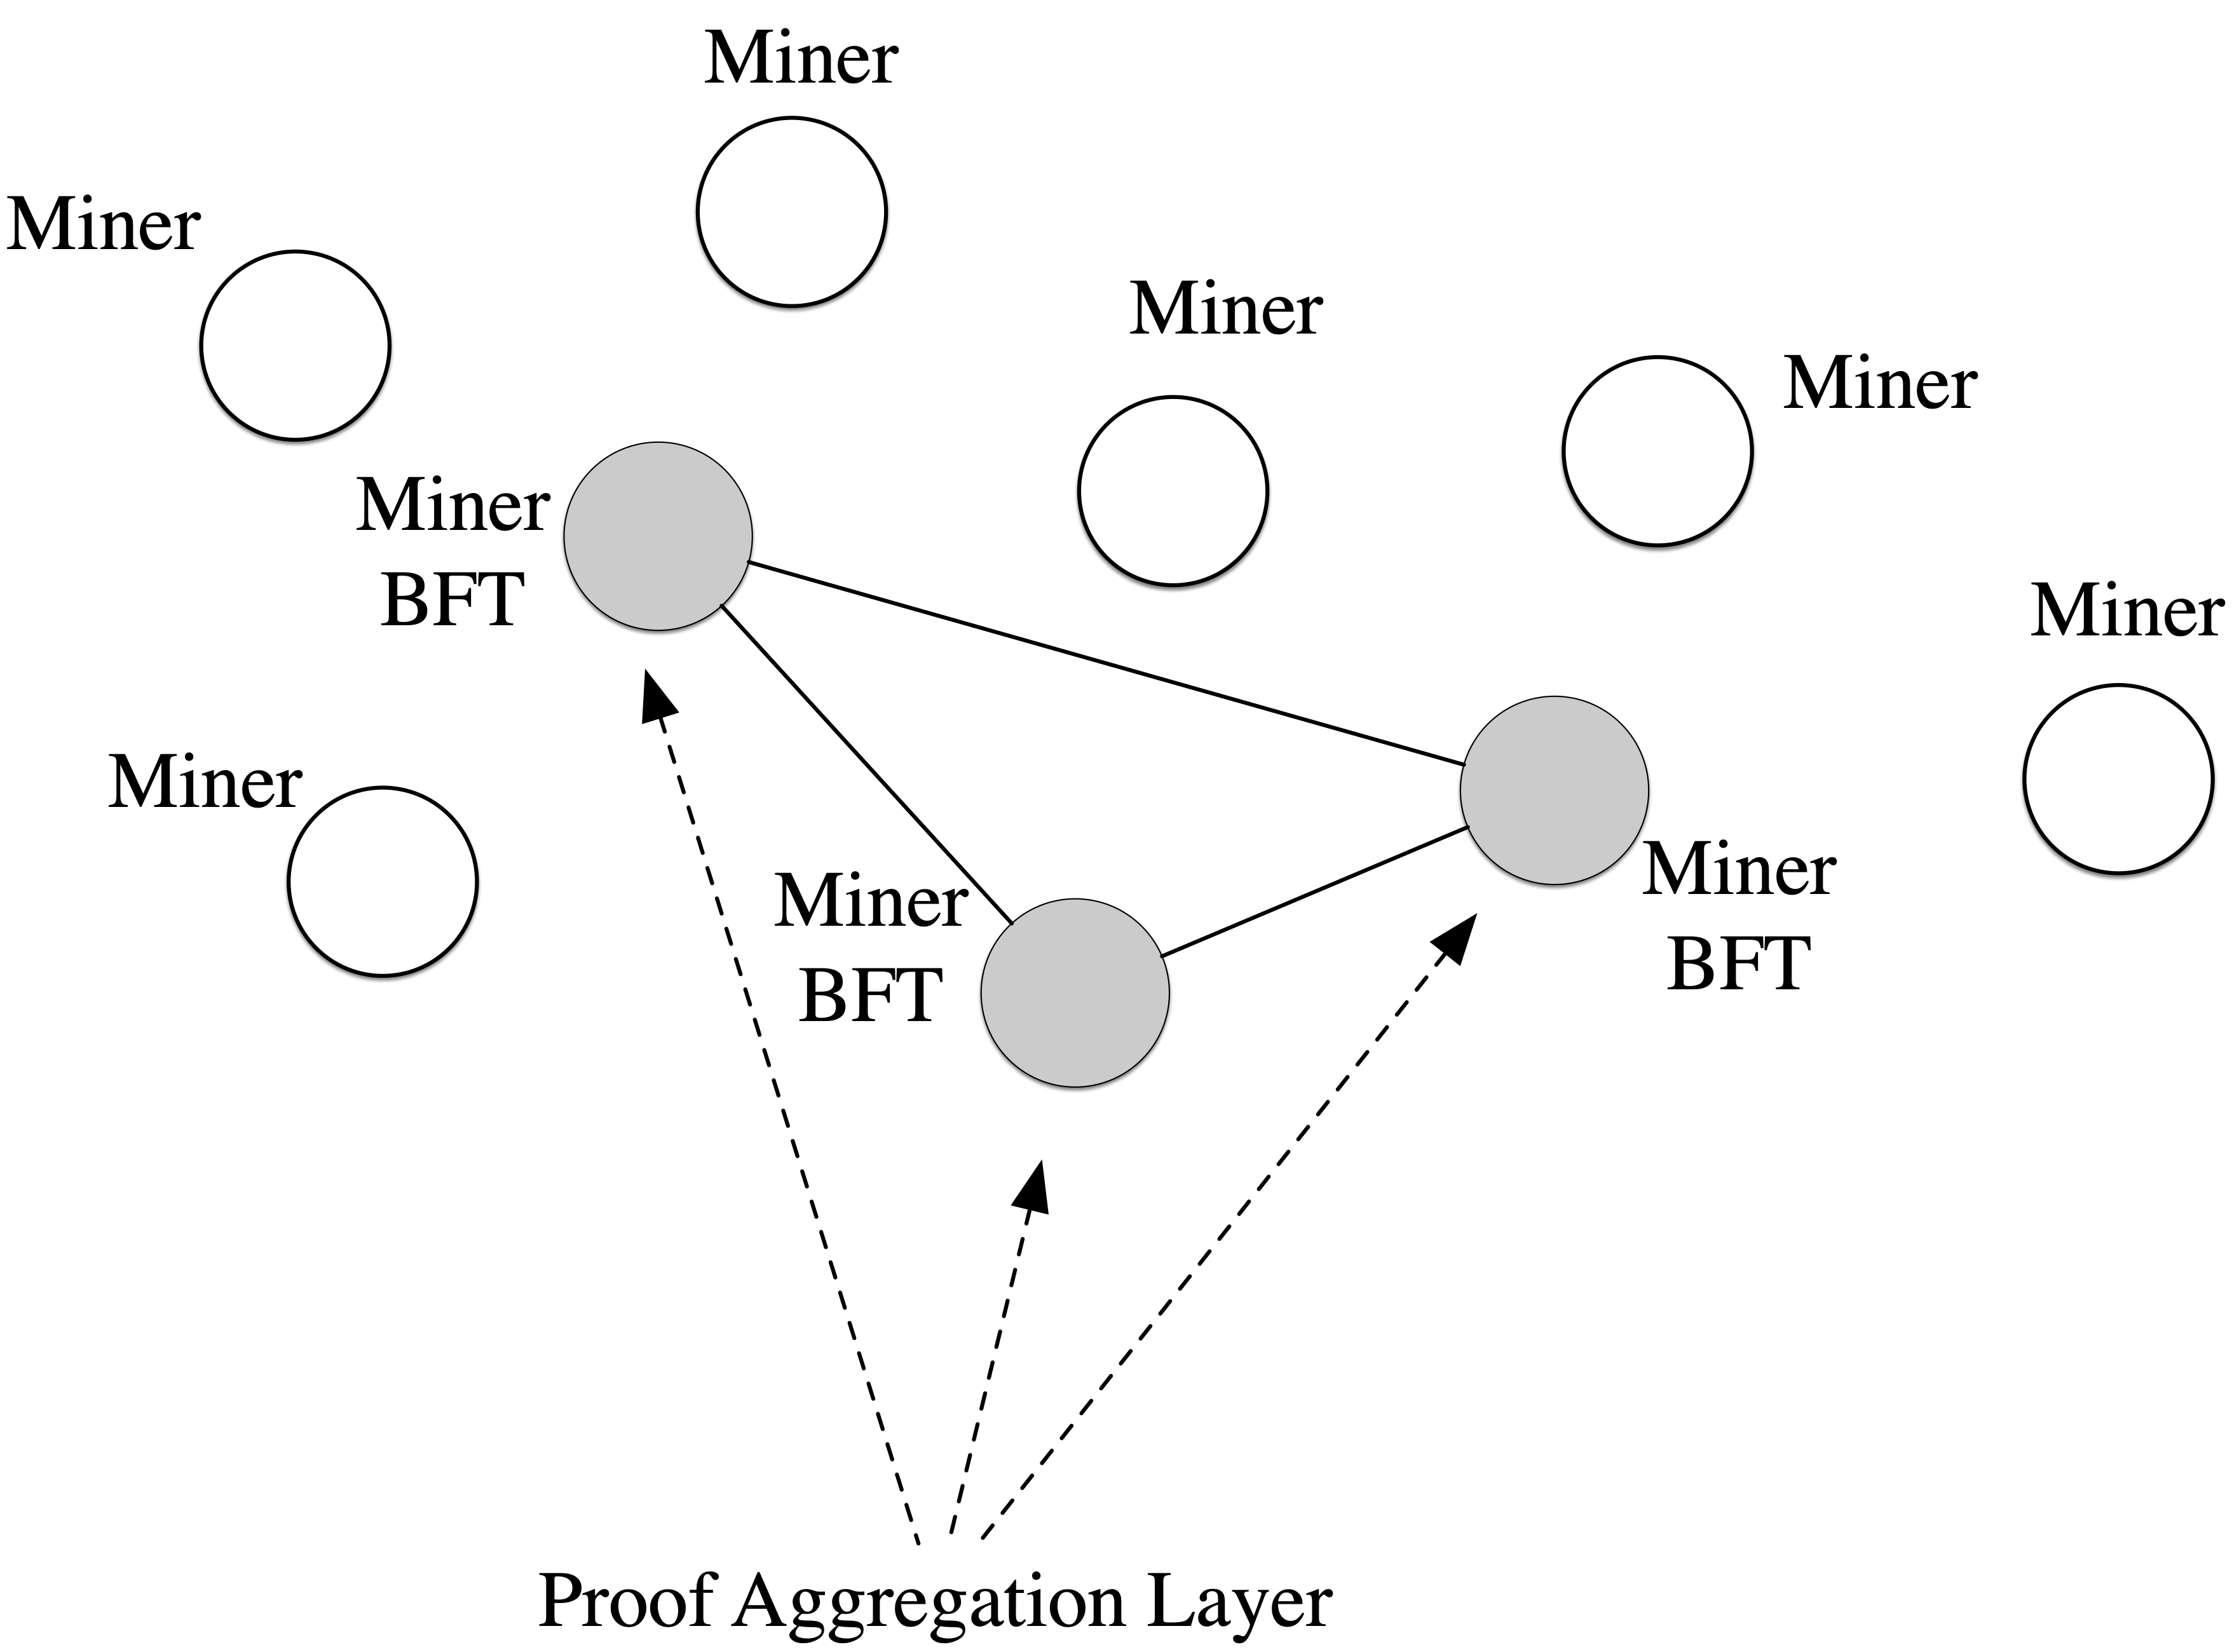
\includegraphics[width=0.7\textwidth]{Miners.png}
    \caption{Consensus Layer with Proof of Work Trust Anchor}
    \label{fig:miners}
\end{figure}

\begin{itemize}
\setlength{\leftmargin}{1em}
 \item Unicity targets two-minute block times and uses RandomX, an ASIC-resistant hashing algorithm. 
 \item A subset of miners, based on winning past block rewards, self-select to operate a BFT consensus subnet operating at one second block times. The BFT subnet implements a finality gadget to periodically ensure settlement finality.
% \item Transactions are restricted to single inputs, enabling the overall ledger to be decomposed into compact individual coin sub-ledgers which can be verified with the same trust assumptions as the full chain.  This allows for the coin sub-ledgers can be extracted from the blockchain and used off-chain, such as for paying transaction fees in Unicity. 
% JVS - I'm not sure what this last sentence means. I also think sub-ledgers deserve a bit more discussion here. For example:
 \item Transactions are restricted to single inputs, enabling the overall ledger to be decomposed into compact individual coin sub-ledgers.  Because each coin is guaranteed to have a single predecessor, it means the full history of that coin can be extracted and verified compactly, without the need to have a copy of the entire chain.  This allows us to create Agents, whose individual actions and correctness can be verified with the same trust assumptions as the full chain.  Additionally, the Agents can be used off-chain, and the work that their use requires can be done in parallel.
\end{itemize}




\subsection*{ASIC Resistance and Fair Mining}

Nakamoto's vision for Bitcoin was based on achieving censorship resistance through decentralization, with the idea that anyone with a computer could participate in the network's consensus mechanism through mining. However, the rapid evolution of mining technology, particularly the development of ASICs, introduced an unforeseen challenge to this egalitarian ideal. These machines, designed solely for the purpose of mining, quickly outpaced general-purpose computer hardware in terms of hash rate, leading to a concentration of mining power. The resulting centralization not only deviated from Bitcoin's original decentralized ethos but also introduced potential vulnerabilities to the network, such as increased susceptibility to 51\% attacks and reduced geographical distribution of miners. 

\vspace{2mm}

In our view, Proof of Work is unsurpassed as means to build a fault tolerant, censorship resistant network. It ties the security of the system to a physical quantity (energy) and with certain limitations, coins can be fairly and transparently distributed. Recently, numerous variations of Proof of Stake as a means to provide a proof of uniqueness. However, the distribution of tokens in Proof of Stake is subject to human oversight leading to errors, malfeasance and fraud. Token allocations and airdrops may give the illusion of decentralization, yet the reality can be quite different. There are certainly limitations to Proof of Work such as potential centralization and slow settlement finality, however these limitations can be overcome with modern technologies. 

\vspace{2mm}

Cryptographers have developed new ASIC resistant hash functions to prevent the centralization of mining power.  RandomX represents the state of the art, and has been battle-tested for several years in Monero, a leading privacy preserving cryptocurrency. Unlike Bitcoin's SHA-256 algorithm, RandomX is designed to be both ASIC-resistant and CPU-friendly.  These attributes level the playing field and help maintain a decentralized network of miners. This democratization not only improves network security through wider participation but also upholds the original Bitcoin vision as a decentralized financial system, accessible to all. RandomX works by generating random code---including a variety of CPU instructions, memory-hard operations and random code execution---that can be efficiently performed by general-purpose processors but are challenging to optimize using specialized hardware. 




\subsection*{Ledger Decomposition}


A simple but key innovation in the Consensus Layer is to restrict UTXOs to single inputs.

\begin{center}
\begin{lstlisting}[language=C++, linewidth=0.8\textwidth]
if (tx.vin.size() != 1)
    return state.Invalid(TxValidationResult::TX_CONSENSUS, 
                         "bad-txns-too-many-inputs", 
                         "Alpha Transactions must have exactly one input");
\end{lstlisting}
\end{center}

Due to the restriction on inputs, it is possible to extract a compact single coin sub-ledger from the ledger and move it off-chain into the agent layer for programmability, scalability and privacy. 
 
\begin{figure}[H]
    \centering
    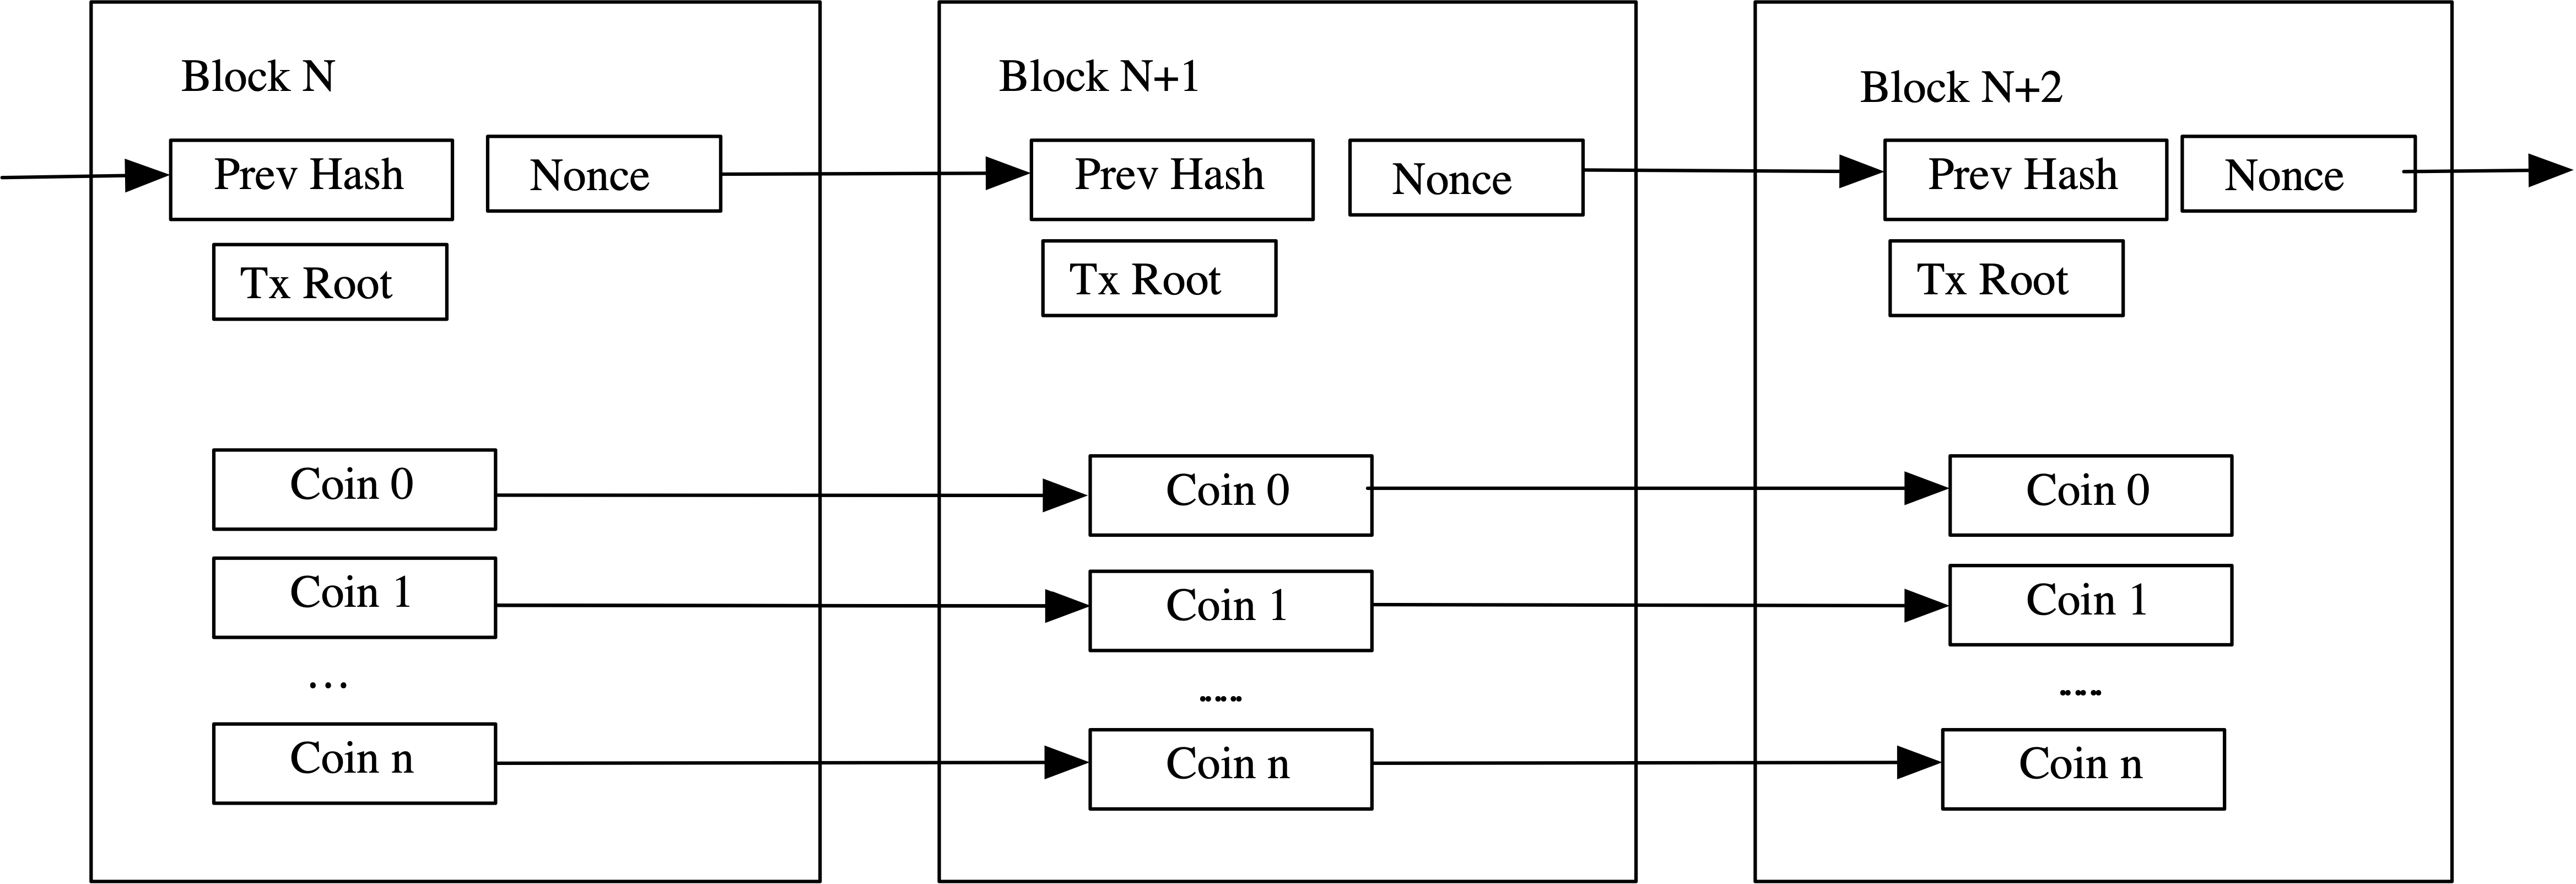
\includegraphics[width=0.8\textwidth]{CoinLedger.png}
    \caption{Decomposition into coin sub-ledgers}
    \label{fig:coinledger}
\end{figure}
\vspace{2mm}

Coin splits (not shown in the diagram above) are allowed as they do not break the local verifiability i.e. the verifiability of a single coin still only depends only on the linear history of that coin and does not require the rest of the ledger or even a substantial part of it.


\section{Implementation: Proof Aggregation Layer}

The Proof Aggregation Layer can be explained in terms of the workflow for an agent to agent interaction. 

\begin{figure}[H]
    \centering
    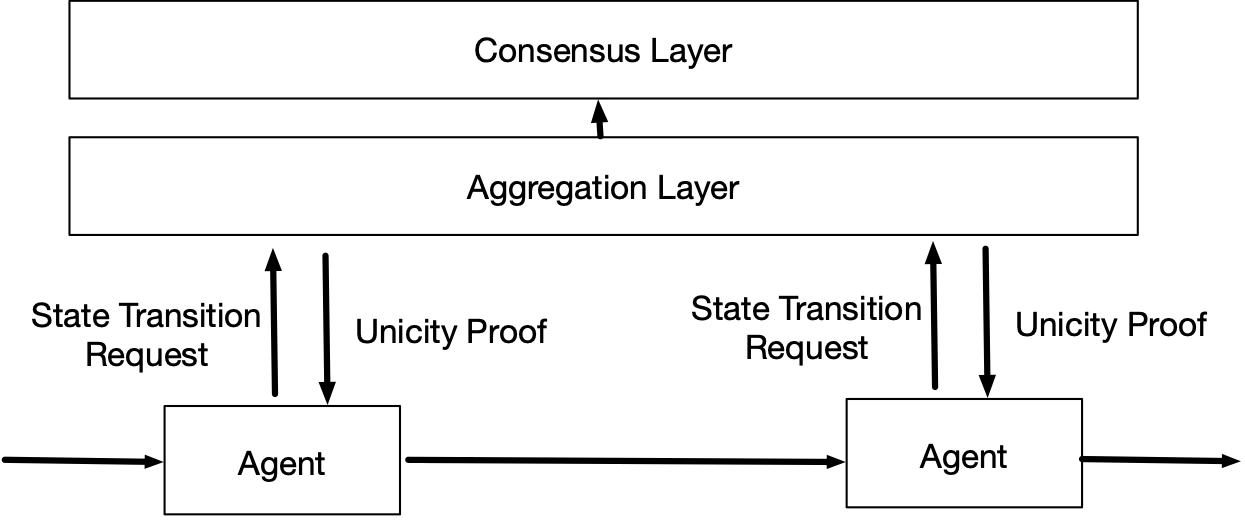
\includegraphics[width=0.6\textwidth]{Workflow.png}
    \caption{Agent to Agent Interaction}
    \label{fig:Workflow}
\end{figure}


An agent will execute locally and send a state transition request to the Aggregation Layer. The Aggregation Layer will generate a Unicity Proof i.e., a proof that shows that the state transition is unique, and return it to the agent who then synchronizes its state with a recipient agent who can verify both the correctness of the agent computation and the uniqueness of the state history.

\vspace{2mm}

\begin{figure}[htbp]
    \centering
    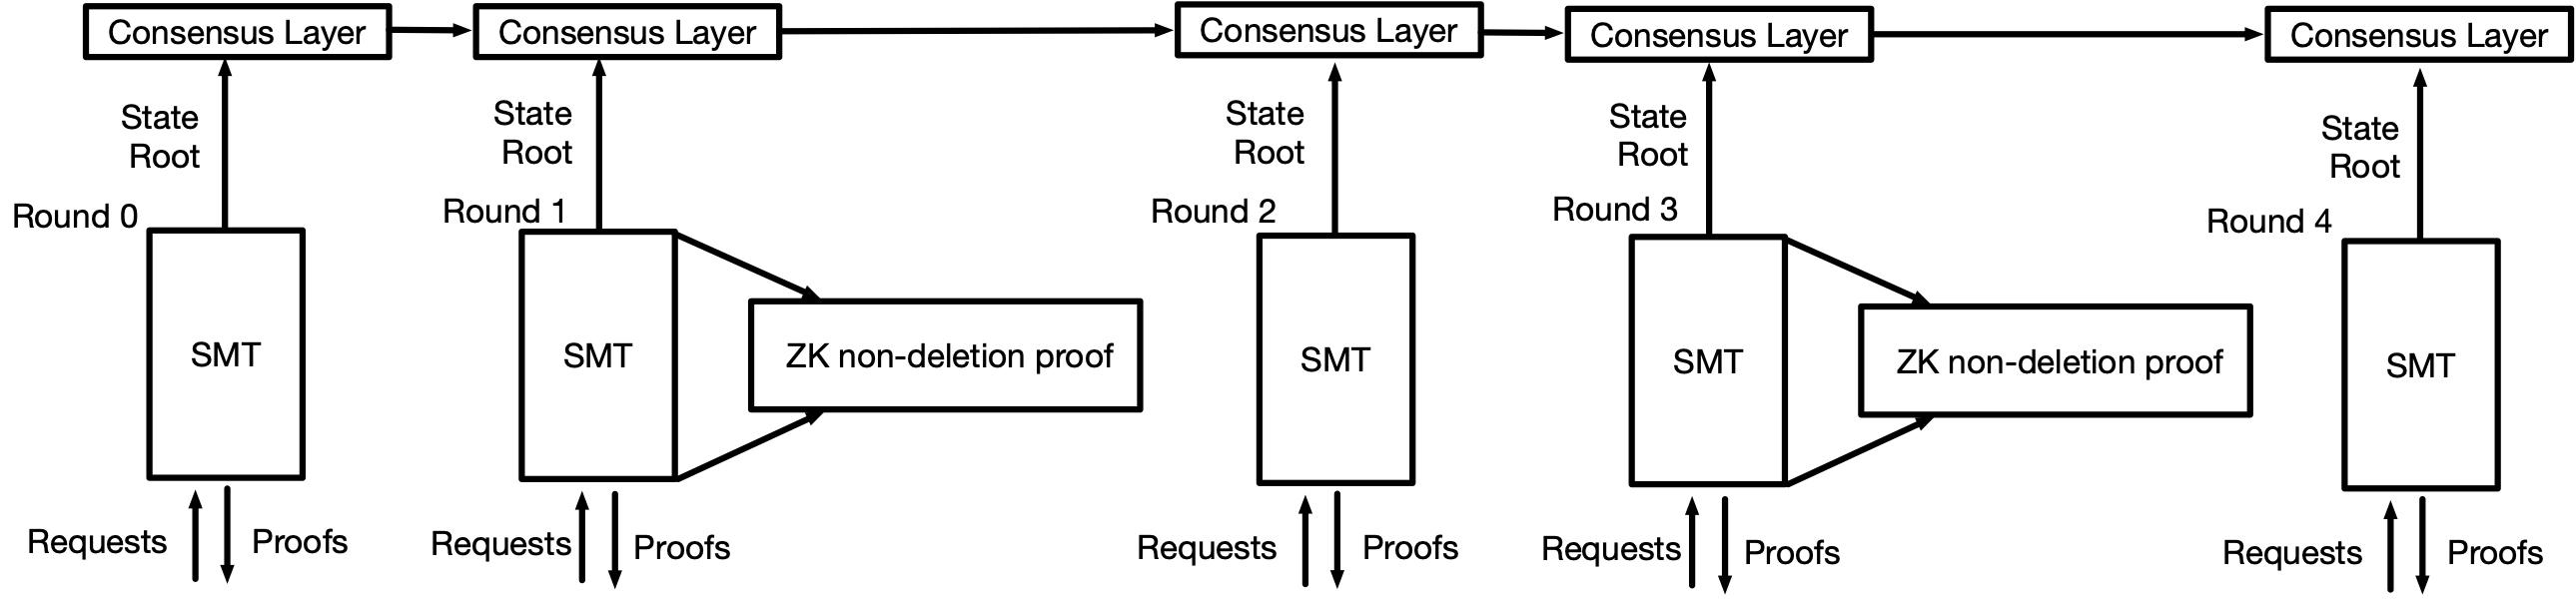
\includegraphics[width=1\textwidth]{SMT.png}
    \caption{Proof Aggregation Layer}
    \label{fig:SMT}
\end{figure}


A Sparse Merkle Tree (SMT) is used such that each unique request is allocated a leaf node in the tree. The details of the request will be described in the next section. A Unicity Proof consists of several elements:
 
 \begin{itemize}
\setlength{\leftmargin}{1em}
\item ZK non-deletion proof at previous ZK checkpoint.
\item Proof of non-inclusion (the SMT hash chain from leaf to root) for all SMT rounds since the previous ZK checkpoint up to the previous round.
\item Proof of inclusion (the SMT hash chain from leaf to root) for the current round.
\end{itemize}


The Aggregation Layer is a decentralized permissionless infrastructure built in a hierarchical manner using smaller sized SMT sub-trees. An Aggregator, or machine that operates a sub-tree or its associated prover is algorithmically assigned a place in the overall infrastructure according to network demand. Aggregators are incentivized to join the network based on transaction fees that are shared across the Aggregator pool. The topology and data structure is designed to be highly redundant and parallelizable i.e. the tree can be dynamically sub-divided into subtrees which operate asynchronously in parallel with redundancy provided by multiple Aggregators processing the same sub-tree.  


\begin{figure}[htbp]
    \centering
    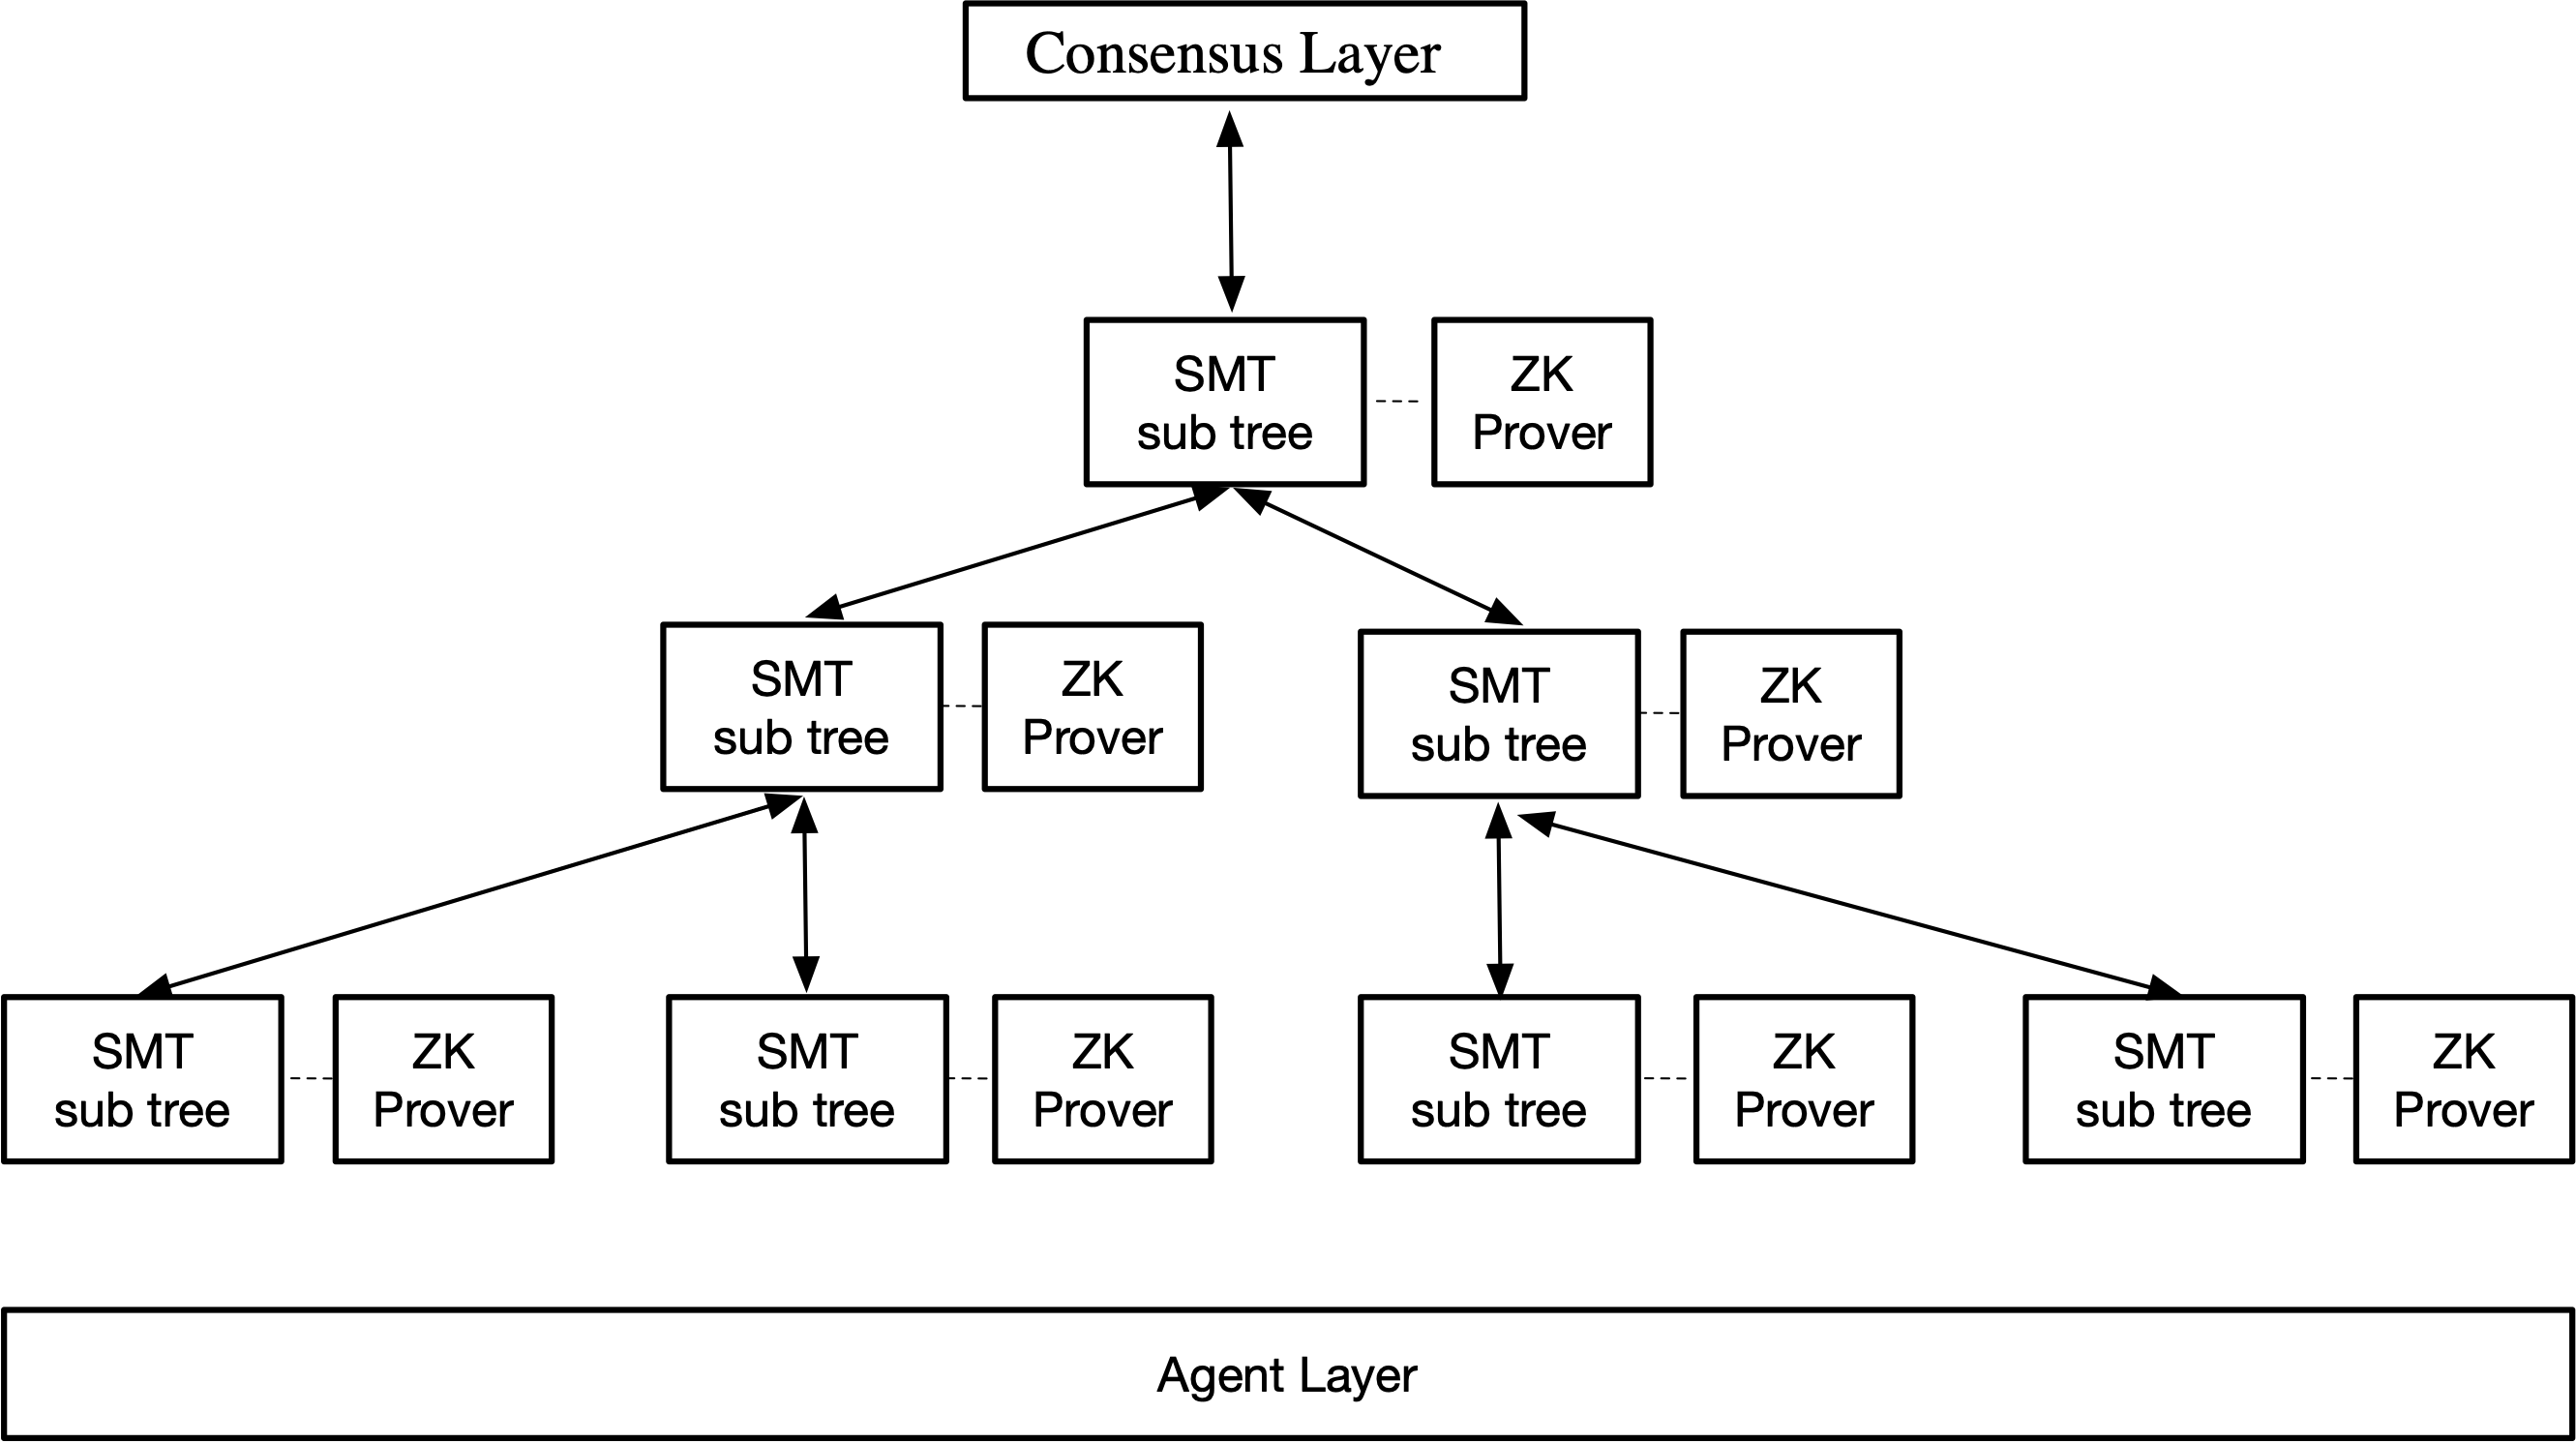
\includegraphics[width=0.6\textwidth]{SMT-Infra.png}
    \caption{Aggregator Hierarchical Infrastructure}
    \label{fig:SMT-Infra}
\end{figure}

\textbf{Dimensioning}
\vspace{2mm}

We assume one million state transition requests per second, EC digital signatures, one second round times, 10 minute ZK checkpoints and 1KB ZK proof size. We assume that the tree remains around a size of 30x$10^{12}$ entries (or 1 million entries per second for an average lifetime of one year) giving a hash-chain size of approximately 1KB.
A Unicity Proof would be at best case 2KB (just after the ZK checkpoint) and at worst case 600KB (just before the ZK Checkpoint\footnote{the size of the proof can be reduced automatically after the next ZK checkpoint.}). 

\vspace{2mm}

There is no bottleneck in the system or centralized points of failure. Subtrees operate asynchronously in clusters and their number and location is algorithmically optimized for network conditions.


\section{Implementation: Agent Layer}


The agent layer provides APIs for developers for agent development, agent to agent communication and interfacing with the Unicity Infrastructure for proof generation. 
\vspace{2mm}

\begin{itemize}
\setlength{\leftmargin}{1em}
\item \textbf{Agent}: an encapsulation of code and state that receives inputs from an external environment, executes its code and updates its state and code accordingly.
\item \textbf{Agent instance}: an instantiation of an agent in an execution environment. Multiple execution environments can share the same agent by synchronizing their agent instances. 
\item \textbf{Token}: an encapsulation of data that has semantic value.
 
\end{itemize}


\textbf{A different programming model}
\vspace{2mm}

We will use the example of a Non Fungible Token (NFT) and highlight the different approach by comparing the operations involved in transferring an NFT in Ethereum and Unicity.  We will assume two users, Alice and Bob. Alice currently owns an NFT and wishes to transfer it to Bob. \vspace{2mm}

In the Ethereum model the NFT exists inside an ERC721 smart contract, which is code and state stored in the Ethereum Blockchain, where the code's execution environment is the Ethereum Virtual Machine (EVM). 

\vspace{2mm}

In Unicity the NFT exists inside an agent, which is code and state which can be stored anywhere.  The agent might exist as multiple instances---each of which execute locally in their own execution environment(s).  This could include Alice's laptop or mobile device, the cloud, at the edge, or all of the above, simultaneously. Unlike Ethereum ERC721 each NFT is implemented by its own agent\footnote{a separate agent may act as minting agent, spawning NFT agents.}.  
\vspace{2mm}

In the Ethereum model Alice will send a transaction order to the blockchain network, which will be received by validators, added to a block proposal and then broadcast to the other validators in the network. Alice and Bob can then verify that the transfer took place by checking that the blockchain includes the transaction.
\vspace{2mm}

In the Unicity model, Alice will send a transaction order to the agent instance in her execution environment that stores the NFT. The agent instance will then execute the transaction order, and request a Unicity Proof from the Unicity infrastructure.  At this point, the transaction has been finalized, and can be synchronized with a new agent instance instantiated in Bob's execution environment. Since the Unicity proof cannot be forged, no alternative transaction history can be claimed for the NFT.  Once synchronized, there are identical agent instances in both Alice and Bob's environments. The agent instance in Bob's execution environment will verify both the Unicity Proof (verifying that there are no forks, i.e. Alice is not trying to double spend) as well as the integrity of computation,\footnote{this could be by simply rerunning the agent code or verifying a ZK proof.} for example, to ensure that the transfer of ownership to his public key has been done correctly.

\begin{figure}[htbp]
    \centering
    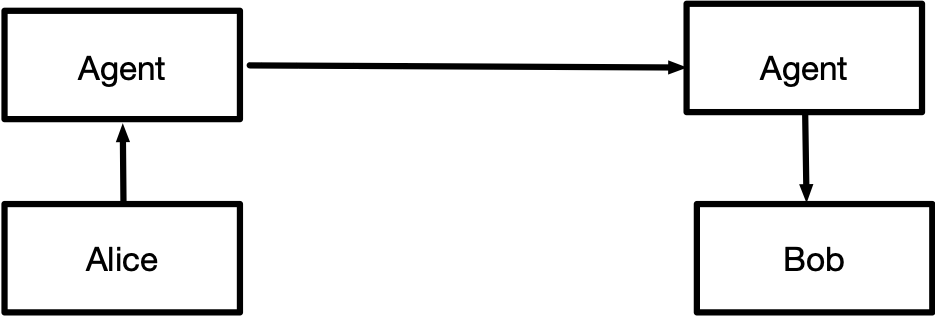
\includegraphics[width=0.4\textwidth]{UserAgent.png}
    \caption{Unicity User Agent Interaction}
    \label{fig:UserAgent}
\end{figure}

At this point, correctly operating agent instances can only accept a valid transaction order from Bob to further transfer the NFT. Alice may choose to delete or archive the agent instance that processed the transaction as it serves no purpose for her going forward\footnote{having multiple copies may of course be useful for censorship resistance or fault tolerance depending on the application.}. 

\vspace{2mm}

The major difference between these two models is that the computational component has been removed from the blockchain, and this allows it to be done in parallel. There may be an unlimited number of agents all interacting with each other or external parties and they do not compete for resources on the blockchain. The blockchain still plays a critical role as the trust anchor but does not play a direct role in execution. The model has changed from a sequential to a parallel programming model.
\vspace{2mm}

\textbf{state transitions}
\vspace{2mm}


The definition of a state transition is agent specific and could be anything from a cryptocurrency transaction, a token mint or player-to-player or agent-to-agent interaction in a multi-player game. In this simple NFT example, we use a very simple configuration for clarity.
\vspace{2mm}

Depending on the application, agents may make use of predicates to change their ownership, code, or data. Predicates are functions that returns a single TRUE or FALSE, used to check if an input meets certain conditions. Predicates are an example of code that can be used by agents to enable customization and programmability. For example, the owner predicate is the function that updates the ownership of an agent, similar to a Bitcoin unlocking script. The most basic form of an owner predicate would be the verification of a digital signature, i.e., in order to transfer ownership, the signature needs to be signed by a private key that matches the public key stored as part of the predicate.
\vspace{2mm}

Different types of predicates may be used to implement various use cases.  A ``data update" predicate allows the user to update a data containing data field in an agents state.  A ``spawn" predicate allows an agent to create new agents and a ``split" predicate allows an agent to subdivide the agent into multiple agents which share characteristics of the parent agent (for example an agent that stores a fungible token).
\vspace{2mm}

We assume that the current state of the NFT agent consists of 

\begin{itemize}
\setlength{\leftmargin}{1em}
 \item  Alice's address, linked to her Public Key.
 \item  An agent ID, created at genesis.
 \item  Data, which in the case of an NFT could be an image or a link to an image.
 \item  Owner  predicate, this is the unlocking condition i.e. only Alice can unlock the owner predicate and transfer ownership.
\end{itemize}

 Similar to standards such as ERC721, the genesis state and allowable state changes are standardized and encoded in the logic of the agent. 

\begin{figure}[htbp]
    \centering
    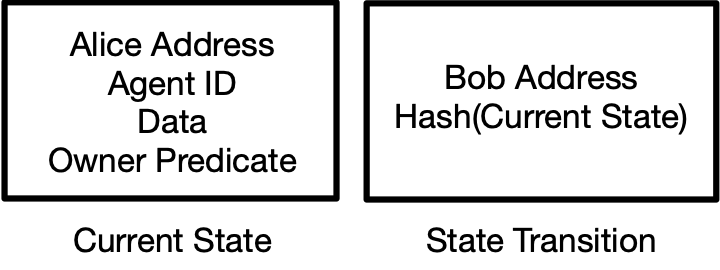
\includegraphics[width=0.3\textwidth]{CurrentStateAndStateTransition.png}
    \caption{Current State and State Transition}
    \label{fig:CurrentState}
\end{figure}

\vspace{2mm}

The first step in the transfer of the NFT to Bob is for Alice to create a state transition. The state transition consists of the hash of the current state and Bob's address. 

\vspace{2mm}
The second step is for Alice to generate a state transition request, a tuple \{RequestID, Payload, Authenticator\}.

\begin{itemize}
\setlength{\leftmargin}{1em}
 \item  \textbf{RequestID} is the address of Alice concatenated with the hash of the current state.
 \item \textbf{Payload} is the hash of the state transition. 
 \item \textbf{Authenticator} is the digital signature of the payload signed by Alice’s private key.
\end{itemize}

The state transition request is then sent to the Unicity Infrastructure where a leaf node is added to the SMT at the address defined by the requestID and content equal to payload plus authenticator. The key point is that there is only one possible requestID for the agent which is registered in the SMT of the Proof Aggregation Layer.

\begin{figure}[H]
    \centering
    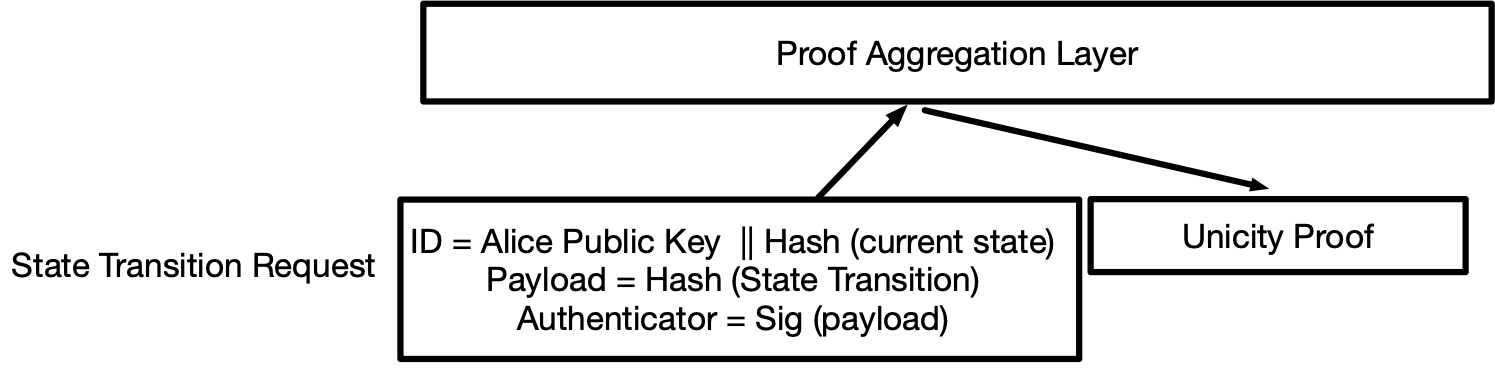
\includegraphics[width=0.6\textwidth]{STR.png}
    \caption{State Transition Request}
    \label{fig:STR}
\end{figure}




Alice's agent instance will then synchronize its state with Bob's agent instance. To verify that Bob is the new owner the agent instance in Bob's execution environment checks that the state transition is valid and that the Unicity Proof verifies that the state transition is unique. Note that the leaf address of the SMT (the RequestID) is defined by the current state and Alice’s public key only.  Any attempt to double spend would required the generation of an identical leaf node address, for which it would be impossible to create a Unicity Proof.

\vspace{2mm}

\begin{figure}[H]
    \centering
    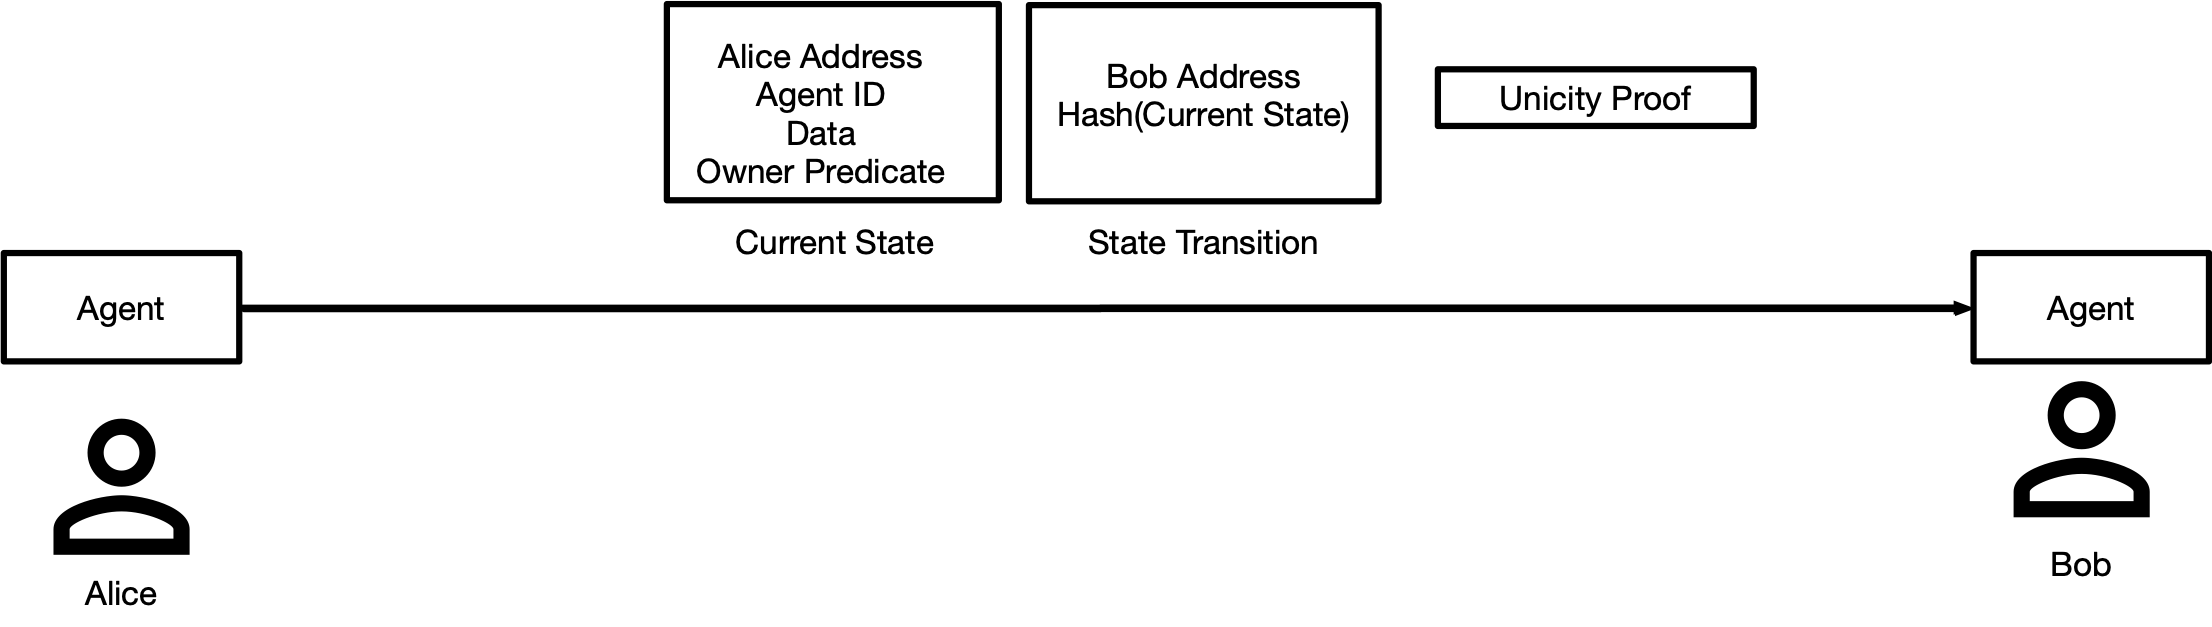
\includegraphics[width=0.7\textwidth]{AgentSynchronization.png}
    \caption{Agent Synchronization}
    \label{fig:AgentSynch}
\end{figure}

\vspace{2mm}

\textbf{programmability and composability}

\vspace{2mm}

The agent model can be extended to include composition, namely different types of agents updating the state of other agents, the splitting of agents, and agents that spawn other agents. In figure \ref{fig:AgentSpawn} we show some example of agents of different types (T1,T2,...). An example of spawning would be an NFT mint agent which is enabled to spawn NFT agents/mint NFTs based on pre-defined conditions. The example of splitting would be agents that are holding state representing some fungible value. If fungibility is allowed as part of the application then an agent may split with the splits each holding part of the overall value. The rules of that application determine how the split should occur, and are implemented in its code. 

\vspace{2mm}

A critical point is that settlement is local i.e. agents do not depend on other agents to execute. All agents are independent and execute locally in their own environments without referring  to other agent's state. This is in contrast to smart contract platforms such as Ethereum in which smart contracts have full access to other smart contracts state, as they all code and state exists within the memory of a single instance of the Ethereum Virtual Machine - which must be small enough to be executed on a single machine, and indeed on a single core. Whilst contracts such as flash loans in Ethereum, i.e. contracts that rely on global state, could be built in Unicity it would reduce the value of the parallelization.


\begin{figure}[H]
    \centering
    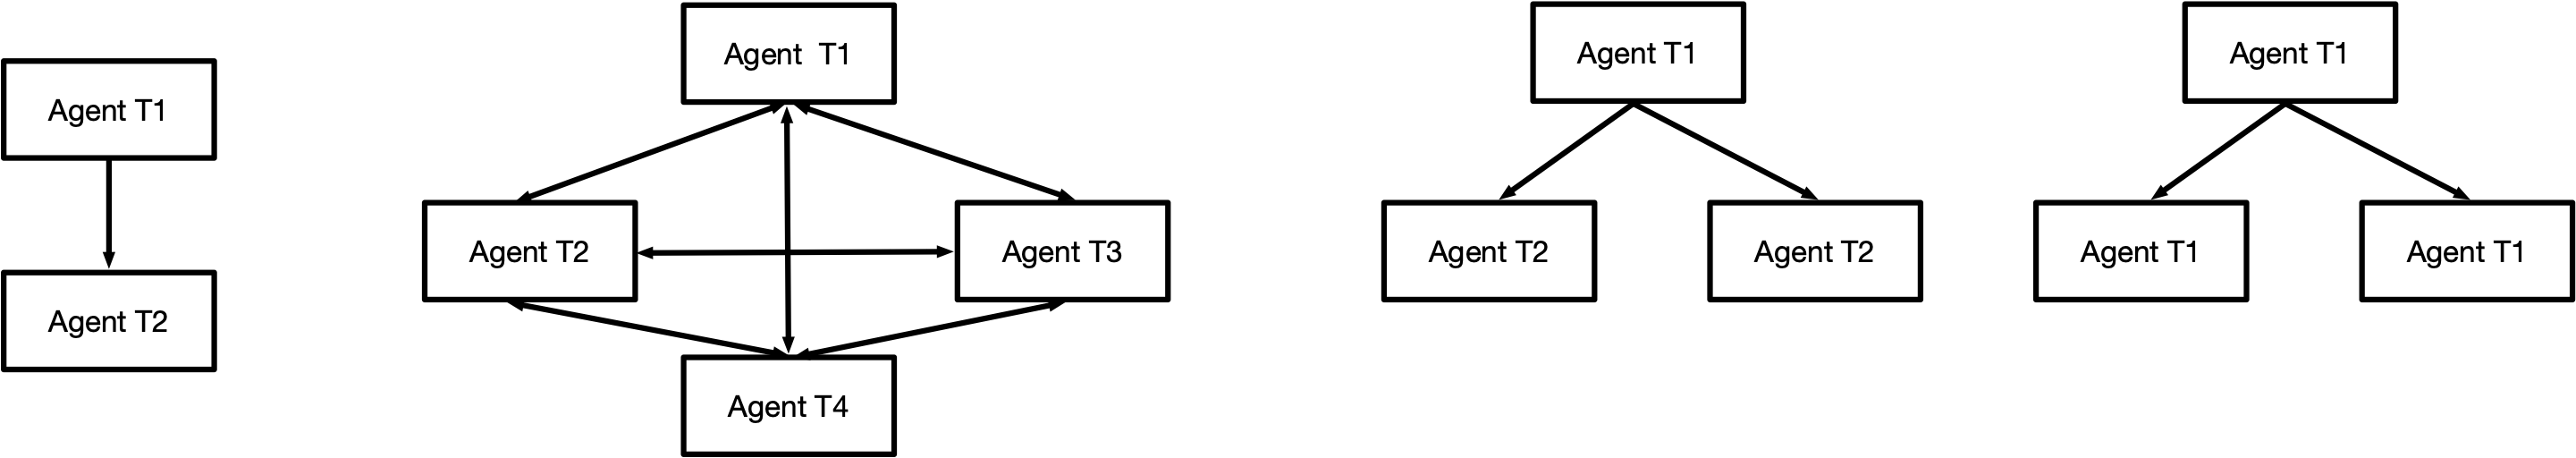
\includegraphics[width=0.9\textwidth]{AgentSpawn.png}
    \caption{Agent Metamorphosis, Agent Composition, Agent Spawning and Agent Splitting}
    \label{fig:AgentSpawn}
\end{figure}



\vspace{2mm}
\textbf{analogy with Kubernetes: an agent approach to DApp deployments}
\vspace{2mm}

The Unicity model is a radical departure from traditional blockchain design, allowing massive scale parallelization of agents which interact to execute a DApp. An analogy with microservices and Kubernetes is relevant. A microservices architecture involves breaking down an application into small, independent services that can be developed, deployed, and scaled independently, with Kubernetes providing the platform for management and orchestration. The Unicity platform involves breaking down a decentralized application into small independent agents that can be developed, deployed and scaled without a centralized gatekeeper. 


\vspace{2mm}
\textbf{zero knowledge: combining verifiable compute and  uniqueness}
\vspace{2mm}

As a result of the increased use of blockchain technologies there has been the surge in research and development of Zero Knowledge (ZK) technology. Zcash pioneered the use of zk-SNARKs (Zero-Knowledge Succinct Non-Interactive Argument of Knowledge) in 2016, enabling fully private transactions on a public blockchain. This breakthrough spurred further innovations, such as Ethereum's implementation of zk-rollups for scalability, reducing transaction costs and increasing throughput. As described earlier, Unicity uses ZK extensively at the Proof Aggregation Layer to provide succinct proofs of non-deletion. ZK techniques can also be applied at the Agent Layer enabling agents to provide verifiable proof of computation to other agents.


\vspace{2mm}


ZK and Unicity solve different problems that when combined represent a powerful approach to building decentralized applications. ZK provides proof of computation but not proof of uniqueness. Many client side ZK proof generation platforms such a Aztec, ZKSync, Aleo etc. can be used in combination with Unicity to provide proof of computation \textbf{and} proof of uniqueness, effectively moving all compute to the client side and reducing the verification task of a recipient to verifying a single ZK Proof. In the simple example above Bob's agent instance must re-execute the state transition to verify the correctness of computation. If Alice's agent generated a ZK Proof of the state transition, it would reduce the work necessary for Bob's agent instance, and also for future recipients of the NFT, to verify the correctness of previous computations.



\section{Programmable Digital Currency}

Bitcoin provided a practical implementation of the ideological commitment to freedom, self-sovereignty, and resistance to government censorship.  It marked a significant advance towards censorship-resistant money with predictable and transparent issuance rules, preventing the kinds of fiscal mismanagement that are inevitable under fiat systems. However, whilst it has proven to be a resilient store of value, it has not seen widespread adoption as a medium of exchange. In this section we show how the Proof of Work coins generated in the Consensus Layer can be extracted and used by agents to provide a highly portable medium of exchange similar to physical cash.

\vspace{2mm}

Alice, is the owner of an Alphacash coin---a coin generated through Proof of Work in the Consensus Layer.  In order to use it like cash, the first step is to transfer the coin to a specified transfer or burn address in the Alphacash ledger. Alice then creates a new agent with a genesis state defined by the transaction ID of the burn transaction in the Alphacash ledger. The agents genesis state includes this transaction ID, the Alphacash coin sub-ledger, and the genesis ownership predicate. The genesis ownership predicate must match the send address in the ultimate transaction in the Alphacash coin sub-ledger i.e. only the private key that initiated the burn transaction can execute a transfer.

\begin{figure}[htbp]
    \centering
    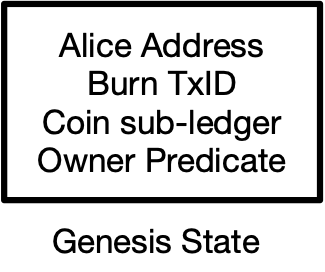
\includegraphics[width=0.15\textwidth]{CoinGenesis.png}
    \caption{Agent Genesis State}
    \label{fig:GenesisEvent}
\end{figure}

The reason for including the Alphacash coin sub-ledger is local verifiability. If a recipient had access to a full node of the PoW blockchain they would have the full history and be able to verify the transaction integrity themselves. However this is quite restrictive and would limit the choices for execution environments. By including the coin sub-ledger a recipient simply needs the genesis block of the PoW blockchain to independently verify the integrity of the coin sub-ledger. The analogy with physical cash is relevant. When someone hands over cash the recipient does not need to verify the integrity of every transaction in history to know that the cash is valid. In other words Unicity agents share the same property of physical cash that verification and settlement happen locally. 
\vspace{2mm}

When Alice wishes to initiate a transfer she will create a state transition and a state transition request similar to the NFT example above. In this case, the token is fungible which means that for transfer of an amount that is less than the value of the coin, the agent will split into two agents, one with the value of the transfer and the other with the value of the remainder or ``change."

\begin{figure}[H]
    \centering
    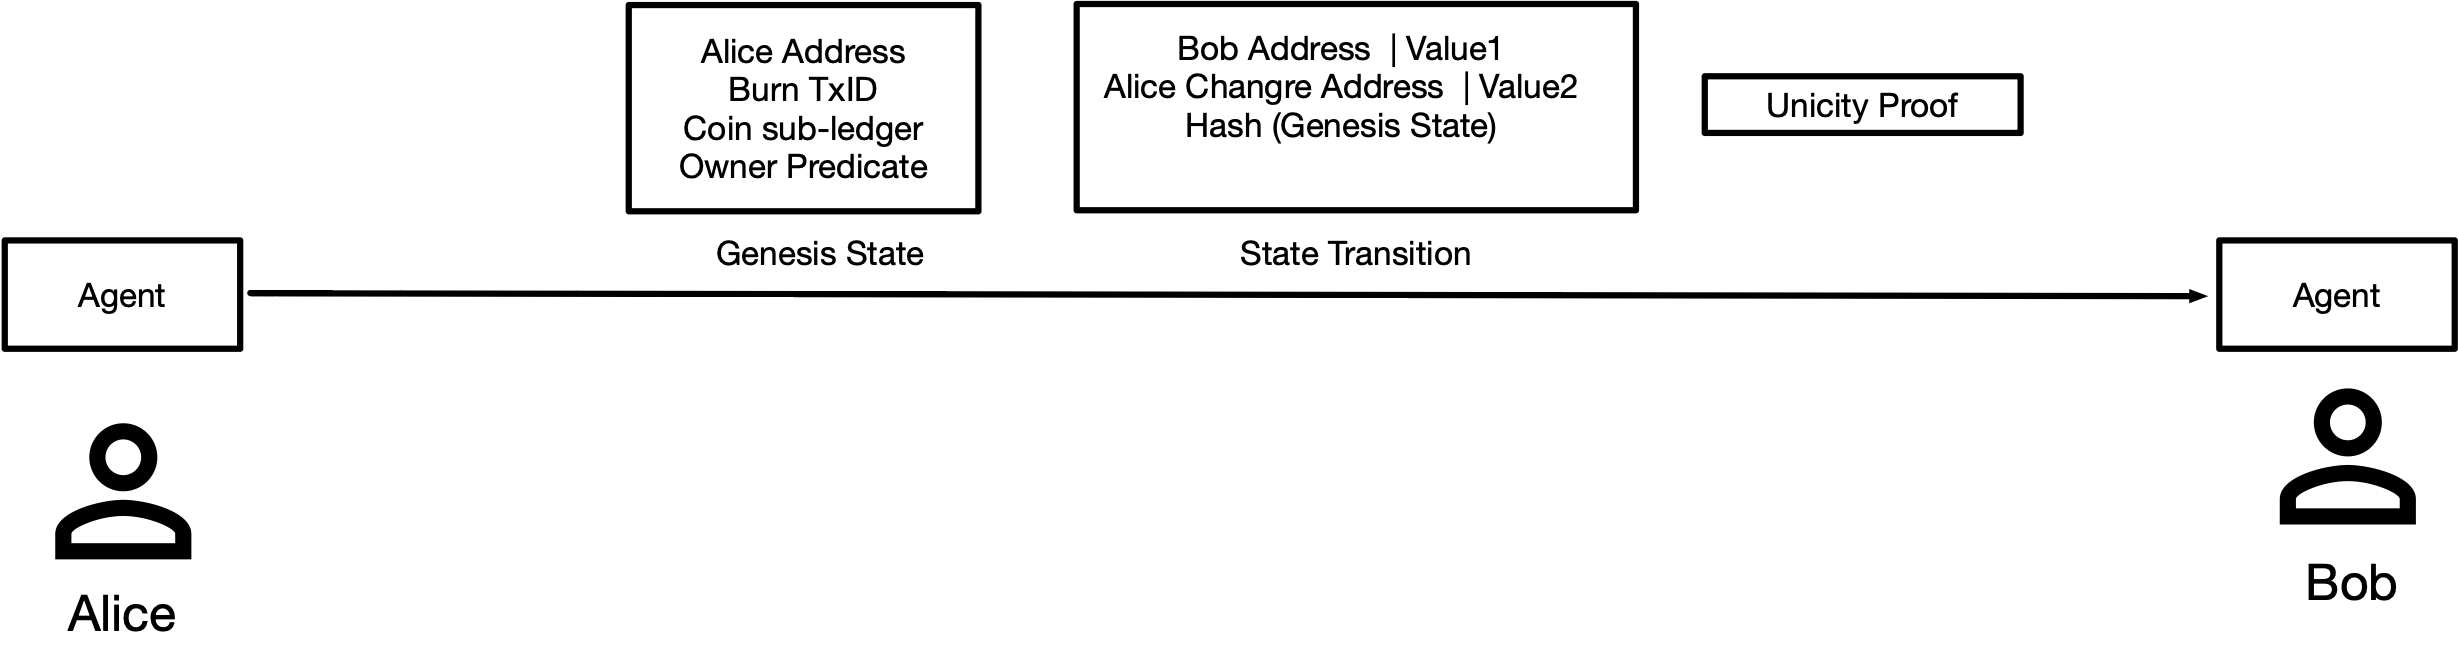
\includegraphics[width=0.9\textwidth]{Alice-Transfer.png}
    \caption{Transfer of a coin minted in the Contract Execution Layer}
    \label{fig:Alice Transfer}
\end{figure}


\vspace{2mm}

Bob's agent will verify the integrity of the Alphacash coin sub-ledger (verifying the burn transaction) as well as the integrity of the state transition and the Unicity Proof. At this point only Bob's agent can execute a transaction order i.e., Bob is now under full control of the agent and therefore the underlying value of the coin.
% It doesn't seem obvious to me how the resulting coin that exists in the Agent's code and state is equivalent to the original coin, where the state was in the Alphacash coin sub-ledger. Ideally, this example would continue to demonstrate how Bob's fully controlled agent can be used to obtain ownership of a coin of equivalent value on the main sub-ledger.  I would write it, but I don't know how it works.

\vspace{2mm}


\section{Decentralized Finance}
There are two compelling reasons for decentralized finance (DeFi). For individuals, the appeal is freedom. The elimination of intermediaries, allowing direct engagement in financial transactions without relying on centralized entities such as banks or payment processors. This provides greater financial autonomy and protection against authoritarian government censorship, ensuring the freedom to transact and access financial services without external control or intervention. For institutions, incorporating elements of DeFi can enhance security and automation by eliminating the need for human oversight. Processes can be streamlined, operational costs reduced, and risks associated with human error or fraud mitigated, while enforcing regulatory compliance at the code level. While these are two very different perspectives, it is clear that DeFi has the potential to revolutionize financial services, driving innovation and empowerment at both the individual and institutional levels.

\vspace{2mm}

While significant progress has been made in productizing DeFi and enhancing the user experience, much work remains. Just as no one is currently running Call of Duty or fully self-driving software in a smart contract today, no one is operating the New York Stock Exchange (NYSE) on a smart contract either. The agent-based approach of Unicity offers a potential path forward by breaking down the components of an exchange into independent agents that execute in parallel. 

\begin{figure}[H]
    \centering
    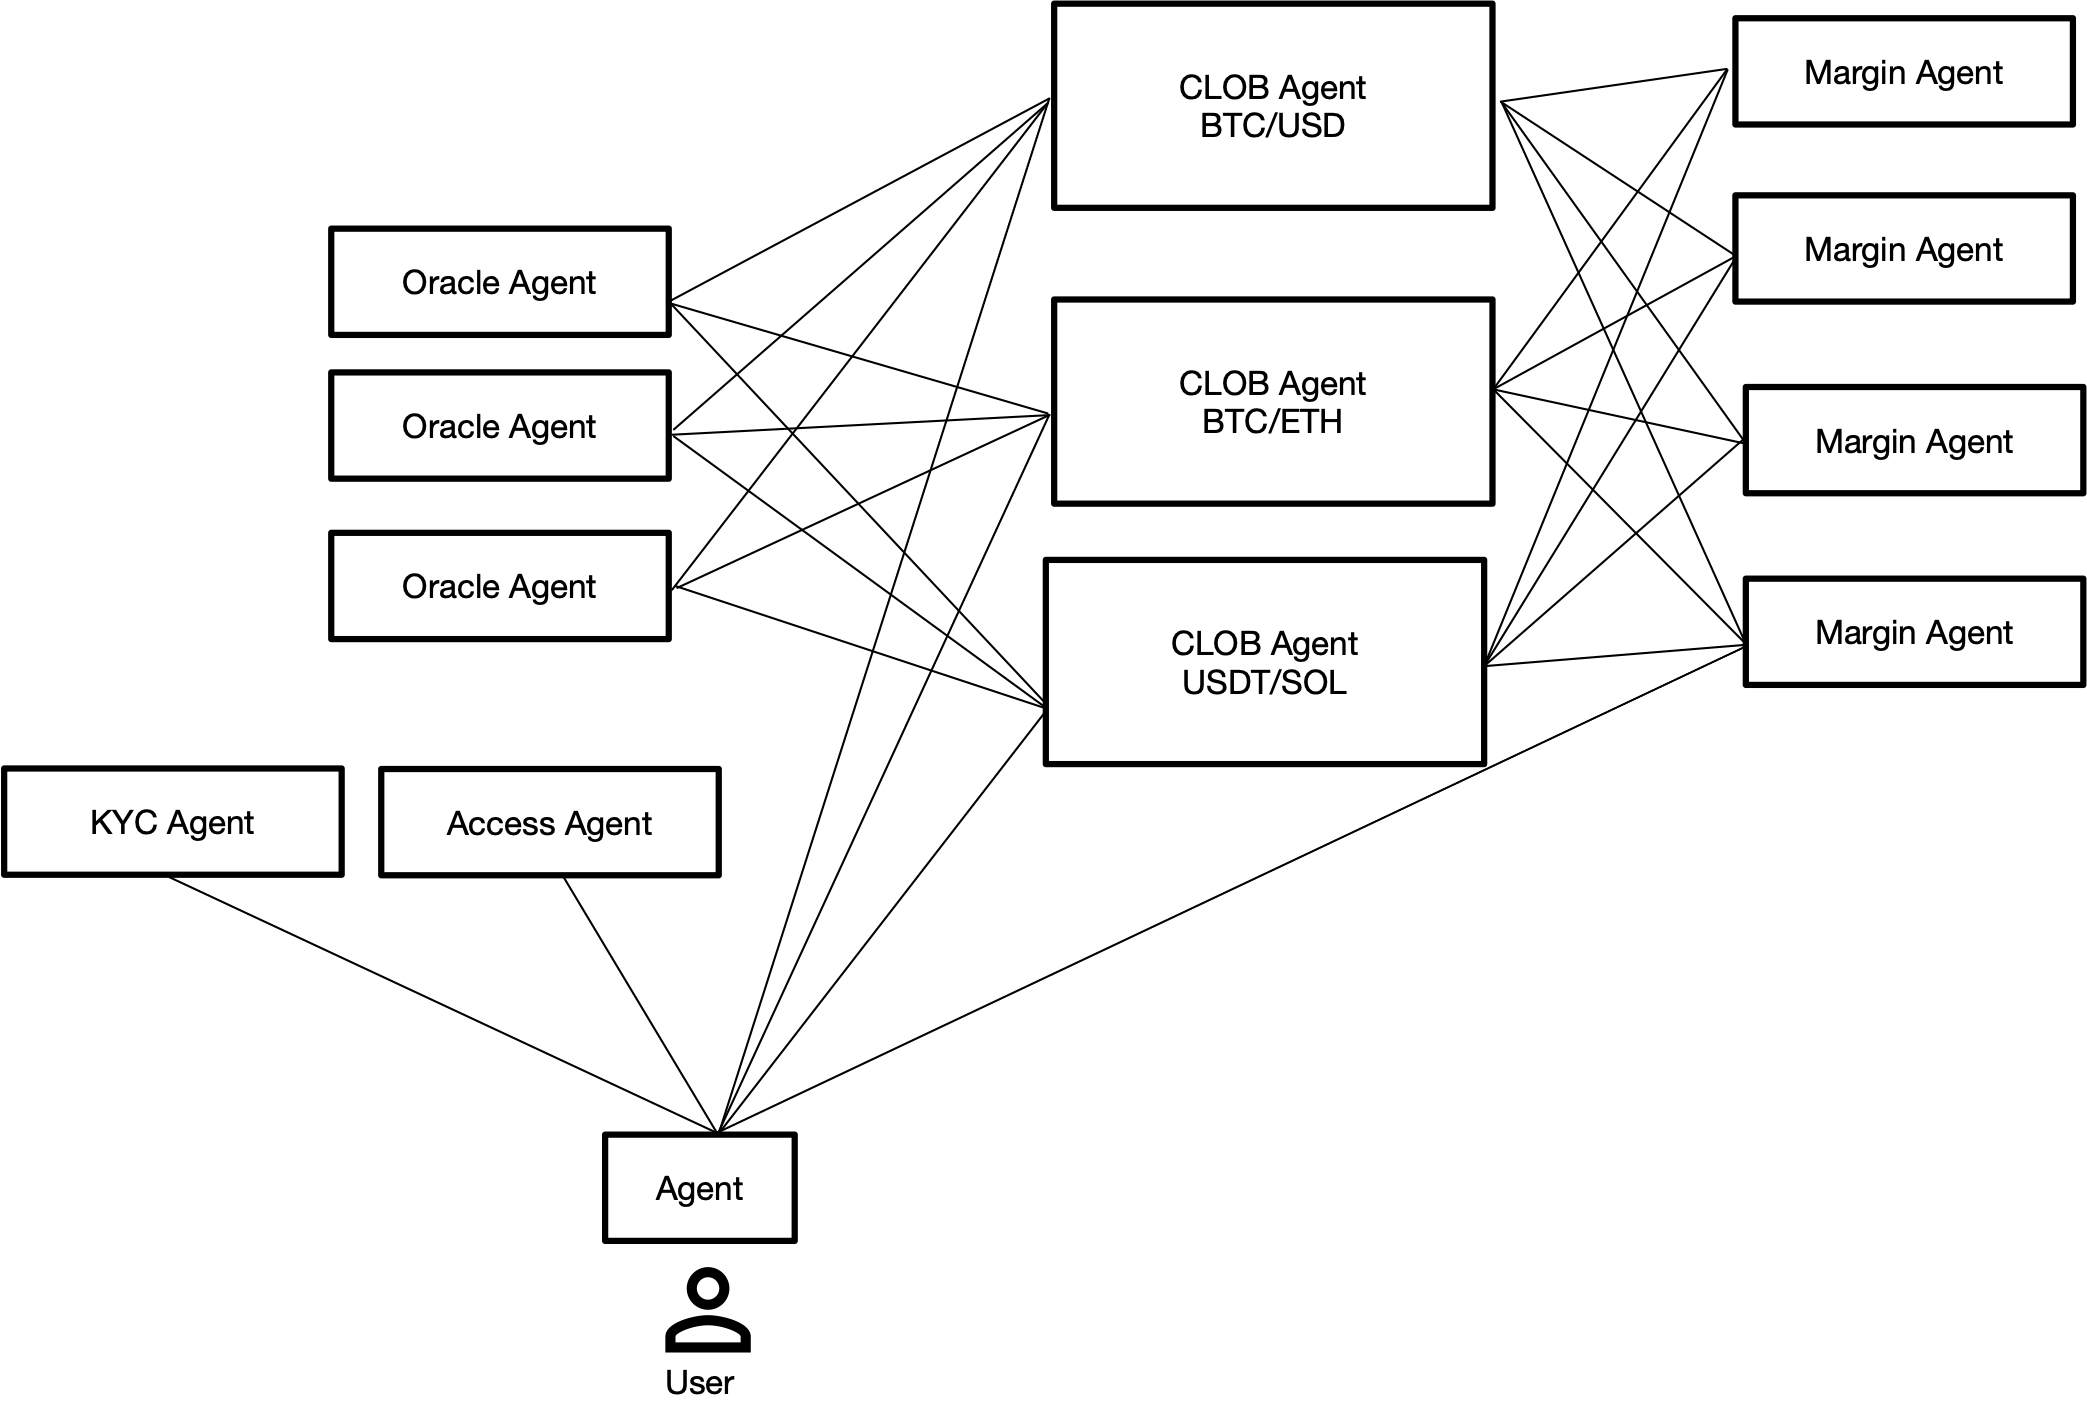
\includegraphics[width=0.7\textwidth]{ABEX.png}
    \caption{Agent-Based Decentralized Exchange}
    \label{fig:ABEX}
\end{figure}

 
Figure \ref{fig:ABEX} shows a simplistic view of a decentralized exchange built using a set of interacting agents. The core agents are the Central Limit Order Book (CLOB) agents which manage individual trading pairs. Depending on requirements these can be deployed and replicated on consumer laptops for a fully permissionless censorship resistant network, or operating in high powered servers in high availability data centers. From a functional perspective, the end result is the same. Individual agents execute in parallel, and synchronize state in a fully transparent, verifiable, and autonomous way. Other agents provide KYC access, margin management, act as price oracles and provide any other functionality that is required to operate the exchange. 


\section{Decentralized Gaming}

Although blockchain technology has been proposed as a means of enhancing transparency and facilitating value exchange in gaming, its current application has largely been limited to asset tokenization within centralized game architectures. Due to the limitations of existing designs, using blockchain for actual game execution remains impractical. However, the potential benefits of decentralized gaming are clear: players can gain true ownership of interoperable assets across different games, enjoy transparency and community-driven governance, experience censorship resistance, unlock innovative business models like play-to-earn, and support fair reward systems for creators.

\vspace{2mm} 
The motivation behind this work came from a desire to solve a real problem in the gaming industry. The industry has, to a large degree, converged on a client-server approach and while the accepted view is that while pure client-side execution of multi-player games is technically possible, it considered impractical due to issues of security, synchronization and scalability. 
\vspace{2mm}

Unicity is an attempt to overcome these limitations and build a truly decentralized game engine for massive online multi-player immersive simulations. In this case decentralization is not a “nice to have” but an essential requirement to allow complex multi-player interactions with potentially millions of players all interacting online. Moving execution to the client side would allow the system to scale, with blockchain technology providing a security layer that guarantees honest gameplay. 

\vspace{2mm}
A user will initiate a set of agents that represent the game: ambience, environment initialization, game mechanics, NPCs etc. as well as agents for in-world or real-world assets. As users interact with the virtual world and approach other players, the players' agents will synchronize with each other with verifiable state transitions proving that the game logic has been followed and enabling the transfer the of assets or currency. 

\begin{figure}[H]
    \centering
    \includegraphics[width=0.5\textwidth]{3Player.png}
    \caption{Three player simulation}
    \label{fig:Threeplayer}
\end{figure}

In the event of a failed verification action can be taken defined by the game logic, such as rewinding the game to the previous known good state. In this way, a completely new type of game engine can be built with the game components consisting of either autonomous agents managing game logic and semi-autonomous agents operating on behalf of the player and interacting with the environment and other players.

\end{document}
